\section{Types of Learning} % (fold)
\noindent
{\color{LightRubineRed} \rule{\linewidth}{1mm} }
\begin{itemize}
\item \textbf{Binary classification}:\par
patient features $\Rightarrow$ sick or not 
\begin{align}
\mathcal{Y} = \{-1,+1\}
\end{align}
\item \textbf{Multiclass Classification}: \par
pathent features $\Rightarrow$ which type of cancer 
\begin{align}
\mathcal{Y} = \{1,2,...,K\}
\end{align}
\item \textbf{regression}: \par
pathent features $\Rightarrow$ how many days before recoverry 
\begin{align}
\mathcal{Y} = \mathbb{R}
\end{align}
\item \textbf{Sequence Learning}: \par
NLP
\end{itemize}
\begin{center}
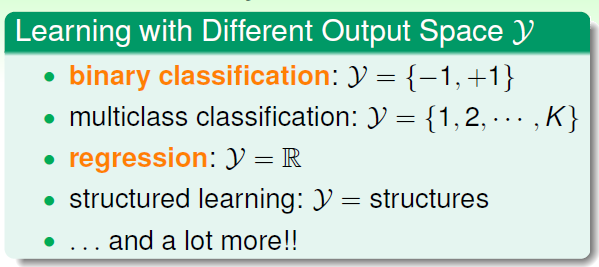
\includegraphics[width=10cm, height=5cm]{lecture3_1}\\
\end{center}
% section section_name (end)
\noindent
{\color{LightRubineRed} \rule{\linewidth}{1mm} }
\begin{itemize}
\item Supervised \par
\item Unsupervised \par
\item Semi-supervised \par
\item Reinforcement
\end{itemize}
\begin{center}
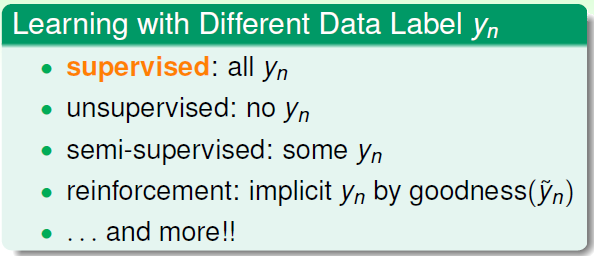
\includegraphics[width=10cm, height=4.5cm]{lecture3_2}\\
\end{center}
输入,输出,训练模式,算法类型。
\begin{center}
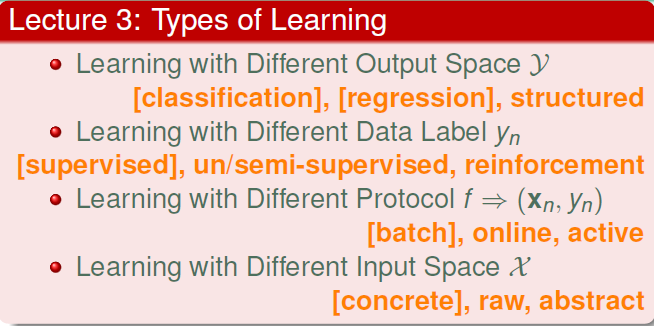
\includegraphics[width=10cm, height=5cm]{lecture3_sum}\\
\end{center}
\noindent
{\color{RubineRed} \rule{\linewidth}{1mm} }